\documentclass{../../algblatt}

\usepackage{stmaryrd}
\usepackage{tabto}
\usepackage{tikz}
\usepackage{geometry}
\usepackage{extarrows}
\geometry{tmargin=2cm,bmargin=2cm,lmargin=2.3cm,rmargin=2.3cm}

\pagestyle{empty}

\newcommand{\fmini}[2]{\framebox{\begin{minipage}{#1}#2\end{minipage}}}
\makeatletter
\def\underunbrace#1{\mathop{\vtop{\m@th\ialign{##\crcr
      $\hfil\displaystyle{#1}\hfil$\crcr\noalign{\kern3\p@\nointerlineskip}
      \crcr\noalign{\kern3\p@}}}}\limits}
\def\overunbrace#1{\mathop{\vbox{\m@th\ialign{##\crcr\noalign{\kern3\p@}
      \crcr\noalign{\kern3\p@\nointerlineskip}
      $\hfil\displaystyle{#1}\hfil$\crcr}}}\limits}
\makeatother

\renewcommand{\labelitemi}{--}

\begin{document}

\begin{center}\Large \sffamily\textbf{Hauptsatz der Galoistheorie}\end{center}

\emph{Situation:} \tabto{1.85cm}
Sei~$K$ ein Koeffizientenbereich (etwa~$K = \QQ$ oder~$K = \QQ(\sqrt[3]{2})$).
\\
\tabto{1.85cm} Sei~$f(X) \in K[X]$ ein normiertes separables Polynom. \\
\tabto{1.85cm} Seien~$x_1,\ldots,x_n$ die Nullstellen von~$f(X)$.
Sei~$E := K(x_1,\ldots,x_n)$. \\
\tabto{1.85cm} Sei~$G := \Gal_K(x_1,\ldots,x_n)$ die Galoisgruppe der
Nullstellen über~$K$.

\emph{Dann gilt:} \tabto{1.85cm} Die Zuordnung
\[
  \begin{array}{@{}rcl@{}}
    \fmini{0.33\textwidth}{Menge der Untergruppen von~$G$}
    &\xleftrightarrow{\text{\qquad1:1\qquad}}&
    \fmini{0.45\textwidth}{Menge der Zwischenerweiterungen von~$E|K$} \\[1.3em]
    H &\longmapsto&
      E^H := \{ x \in E \,|\, \text{$\sigma(x) = x$ für alle~$\sigma \in H$} \} \\[0.3em]
    \mathrm{Gal}_L(x_1,\ldots,x_n) &\longmapsfrom& L
%   = \{ \sigma \in G \,|\, \text{$\sigma \cdot x = x$ für alle~$x \in L$} \}
  \end{array}
\]
ist eine inklusionsumkehrende Bijektion.
Genauer gilt für alle Zwischenerweiterungen~$L,L'$ von~$E|K$
und Untergruppen~$H,H'$ von~$G$:
\begin{enumerate}
\item $E^{\mathrm{Gal}_L(x_1,\ldots,x_n)} = L$,
\tabto{9cm}$\mathrm{Gal}_{E^H}(x_1,\ldots,x_n) = H$.

\item $L \subseteq L' \Leftrightarrow \mathrm{Gal}_L(x_1,\ldots,x_n)
\supseteq \Gal_{L'}(x_1,\ldots,x_n)$,
\tabto{9cm}$H \subseteq H' \Leftrightarrow E^H \supseteq E^{H'}$.

\item $|H| = \gra{H}{1} = \gra{E}{E^H}$,
\tabto{9cm}$\gra{E^H}{K} = \gra{G}{H} = |G| \mathop{/} |H|.$

\item In Algebra II werden wir eine einfache Charakterisierung dafür
kennenlernen, wann~$H$ ein Normalteiler in~$G$ ist.
\end{enumerate}

\emph{Wie kann man die relativen Galoisgruppen ausrechnen?}
Wenn~$L = K(z_1,\ldots,z_m)$, gilt
\[ \Gal_L(x_1,\ldots,x_n) = \{ \sigma \in G \,|\,
  \text{$\sigma \cdot z_i = z_i$ für~$i = 1,\ldots,m$} \}. \]

\emph{Wie kann man Erzeuger der Fixkörper bestimmen?}
Falls~$H = \{ \sigma_1,\ldots,\sigma_m \}$ und~$E = K(t)$, gilt
\[ E^H = K(
  e_1(\sigma_1 \cdot t, \ldots, \sigma_m \cdot t),
  \ldots,
  e_m(\sigma_1 \cdot t, \ldots, \sigma_m \cdot t)), \]
wobei die~$e_i$ die elementarsymmetrischen Funktionen in~$m$ Unbekannten seien.

\subsection*{Beispiel}

Sei~$L := \QQ(\sqrt{2}, \i)$ der Zerfällungskörper von~$(X^2 - 2) (X^2 + 1)$
über~$K := \QQ$.
\begin{enumerate}
\item Die Galoisgruppe~$G$ besteht aus folgenden vier
Elementen~$\sigma_1,\ldots,\sigma_4$:
\begin{align*}
  \sigma_1{:} & \sqrt{2} \mapsto \phantom{+}\sqrt{2}, \qquad \i \mapsto \phantom{+}\i \\
  \sigma_2{:} & \sqrt{2} \mapsto \phantom{+}\sqrt{2}, \qquad \i \mapsto         {-}\i \\
  \sigma_3{:} & \sqrt{2} \mapsto         {-}\sqrt{2}, \qquad \i \mapsto \phantom{+}\i \\
  \sigma_4{:} & \sqrt{2} \mapsto         {-}\sqrt{2}, \qquad \i \mapsto         {-}\i \\
\end{align*}
\item Die Verknüpfungstafel ist:
\[ \begin{array}{@{}c|cccc@{}}
  \circ & \sigma_1 & \sigma_2 & \sigma_3 & \sigma_4 \\\hline
  \sigma_1 & \sigma_1 & \sigma_2 & \sigma_3 & \sigma_4 \\
  \sigma_2 & \sigma_2 & \sigma_1 & \sigma_4 & \sigma_3 \\
  \sigma_3 & \sigma_3 & \sigma_4 & \sigma_1 & \sigma_2 \\
  \sigma_4 & \sigma_4 & \sigma_3 & \sigma_2 & \sigma_1
\end{array} \]
Dazu sind die Nebenrechnungen $\sigma_2 \circ \sigma_2 = \sigma_1$ und
$\sigma_3 \circ \sigma_3 = \sigma_1$ erforderlich, den Rest kann man nach der
Regel "`in jeder Zeile und Spalte muss jedes Gruppenelement genau einmal
vorkommen"' erschließen.
\item Tafel der Untergruppen von~$G$ und der Zwischenerweiterungen von~$\QQ(\sqrt{2},\i)$ über~$\QQ$:
\begin{center}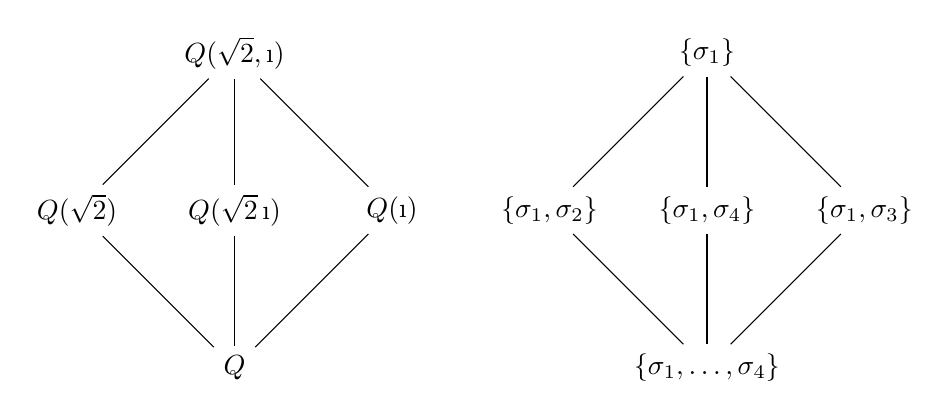
\begin{tikzpicture}[node distance=2cm]
 \node (Q)                  {$\mathbb{Q}$};
 \node (Q6)  [above of=Q]   {$\mathbb{Q}(\sqrt{2}\,\i)$};
 \node (Q2)  [right of=Q6]  {$\mathbb{Q}(\i)$};
 \node (Q3)  [left of=Q6]   {$\mathbb{Q}(\sqrt{2})$};
 \node (Q23) [above of=Q6]  {$\mathbb{Q}(\sqrt{2}, \i)$};
 \node (1f)  [right of=Q2]  {$\{\sigma_1, \sigma_2 \}$};
 \node (1fg) [right of=1f]  {$\{\sigma_1, \sigma_4 \}$};
 \node (1g)  [right of=1fg] {$\{\sigma_1, \sigma_3 \}$};
 \node (G)   [below of=1fg] {$\{\sigma_1, \ldots, \sigma_4 \}$};
 \node (1)   [above of=1fg] {$\{\sigma_1\}$};
 \draw (Q)   -- (Q2);
 \draw (Q)   -- (Q3);
 \draw (Q)   -- (Q6);
 \draw (Q2)  -- (Q23);
 \draw (Q3)  -- (Q23);
 \draw (Q6)  -- (Q23);
 \draw (G)   -- (1f);
 \draw (G)   -- (1fg);
 \draw (G)   -- (1g);
 \draw (1f)  -- (1);
 \draw (1fg) -- (1);
 \draw (1g)  -- (1);
\end{tikzpicture}\end{center}
Im linken Diagramm steht oben die größte und unten die kleinste
Zwischenerweiterung, im rechten Diagramm umgekehrt oben die kleinste und unten die
größte Un\-ter\-grup\-pe der Galoisgruppe. Das ist so gemacht, dass zu einer
Zwischenerweiterung an der entsprechenden Stelle rechts die zugehörige relative
Galoisgruppe und zu einer Untergruppe entsprechend links der zugehörige
Fixkörper steht.

\item Exemplarisch der Nachweis, dass~$L^{\{\sigma_1,\sigma_4\}} =
\QQ(\sqrt{2}\,\i)$:

Die Richtung "`$\supseteq$"' ist klar, da die Zahl~$\sqrt{2}\,\i$
von~$\sigma_4$ (und von~$\sigma_1$ sowieso) festgehalten wird:
\[ \sigma_4(\sqrt{2} \, \i) = \sigma_4(\sqrt{2}) \, \sigma_4(\i) = (-\sqrt{2}) (-\i) = \sqrt{2}\,\i \]
Die andere Richtung folgt aus Gradgründen:
\begin{align*}
  [L^{\{\sigma_1,\sigma_4\}} : \QQ] &= |G|\,/\,|\{\sigma_1,\sigma_4\}| = 4/2 = 2 \\
  [\QQ(\sqrt{2}\,\i):\QQ] &= 2
\end{align*}
\end{enumerate}

\end{document}
